\section{Role\-Manager Class Reference}
\label{classRoleManager}\index{RoleManager@{RoleManager}}
Inheritance diagram for Role\-Manager:\begin{figure}[H]
\begin{center}
\leavevmode
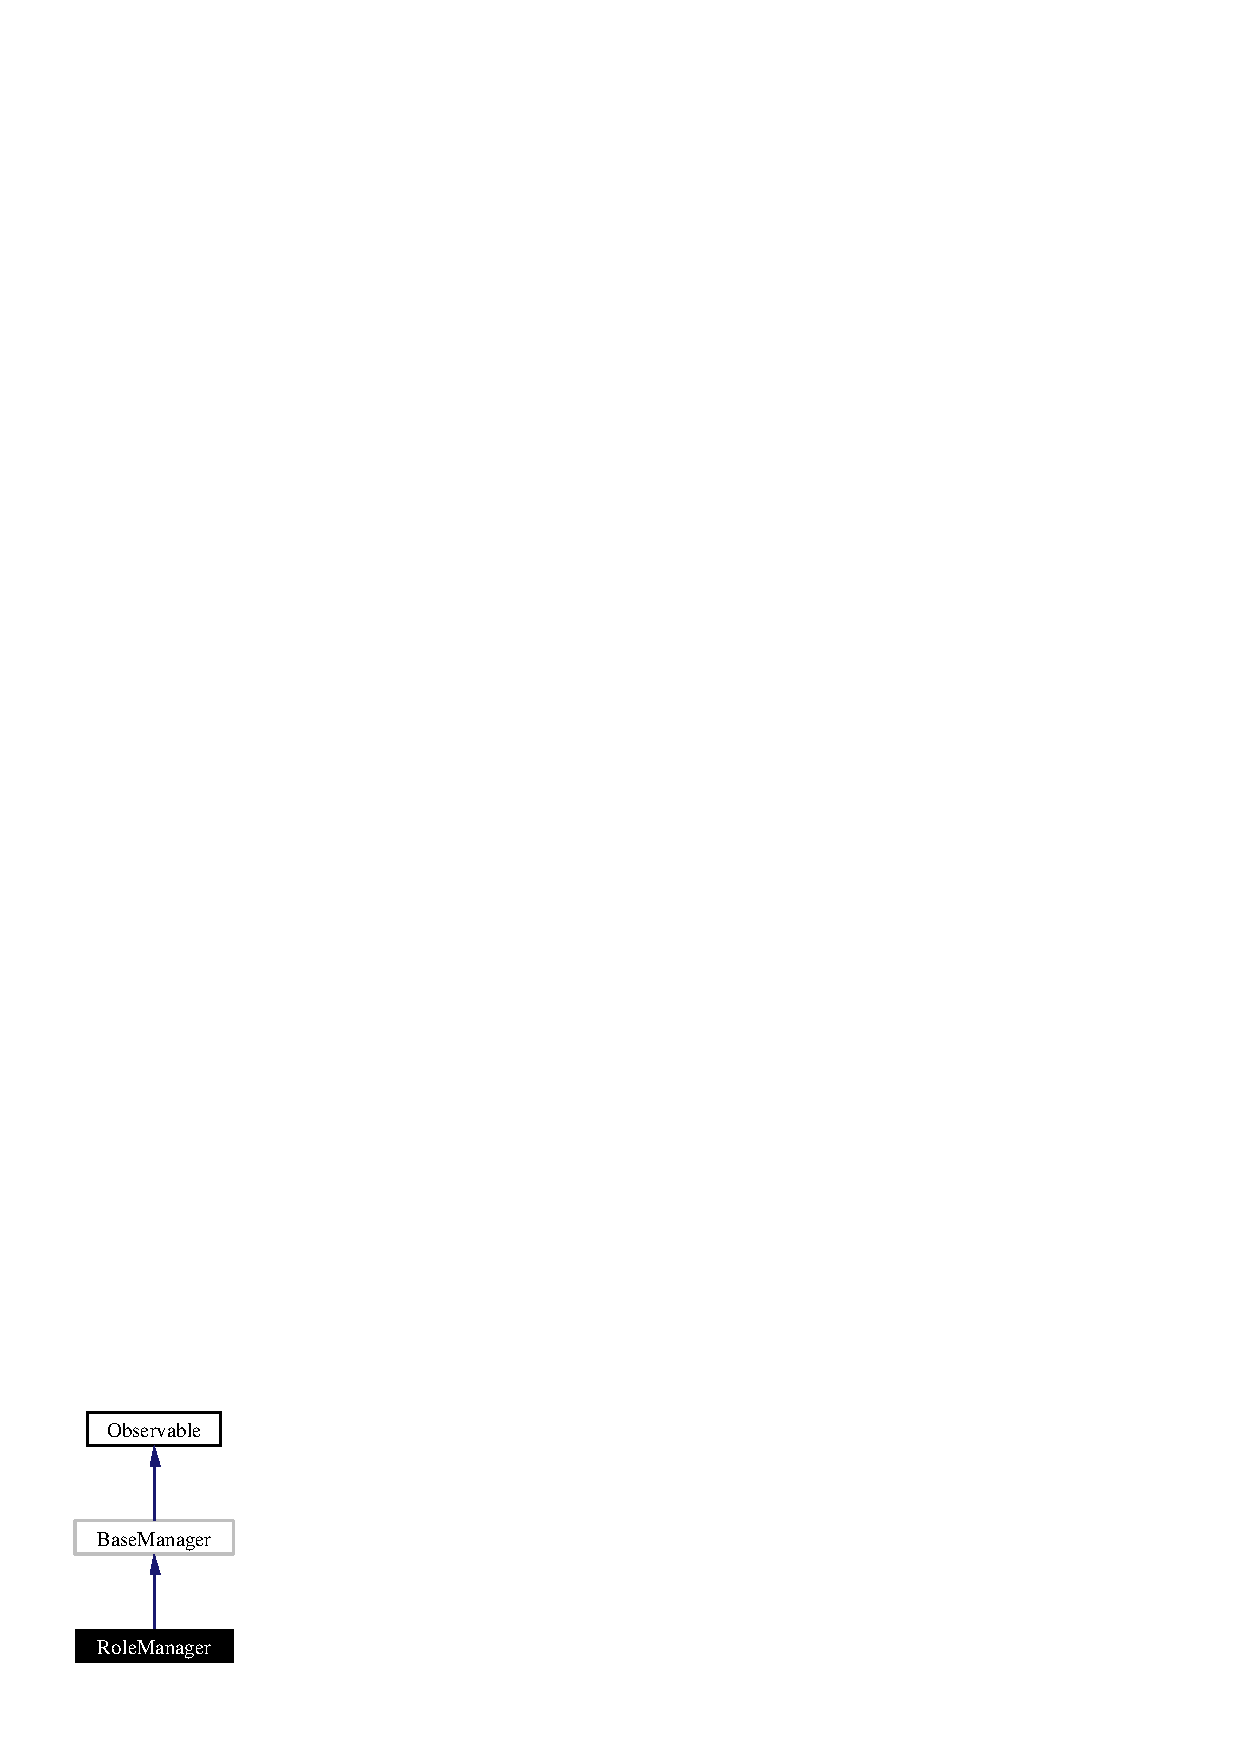
\includegraphics[width=56pt]{classRoleManager__inherit__graph}
\end{center}
\end{figure}
Collaboration diagram for Role\-Manager:\begin{figure}[H]
\begin{center}
\leavevmode
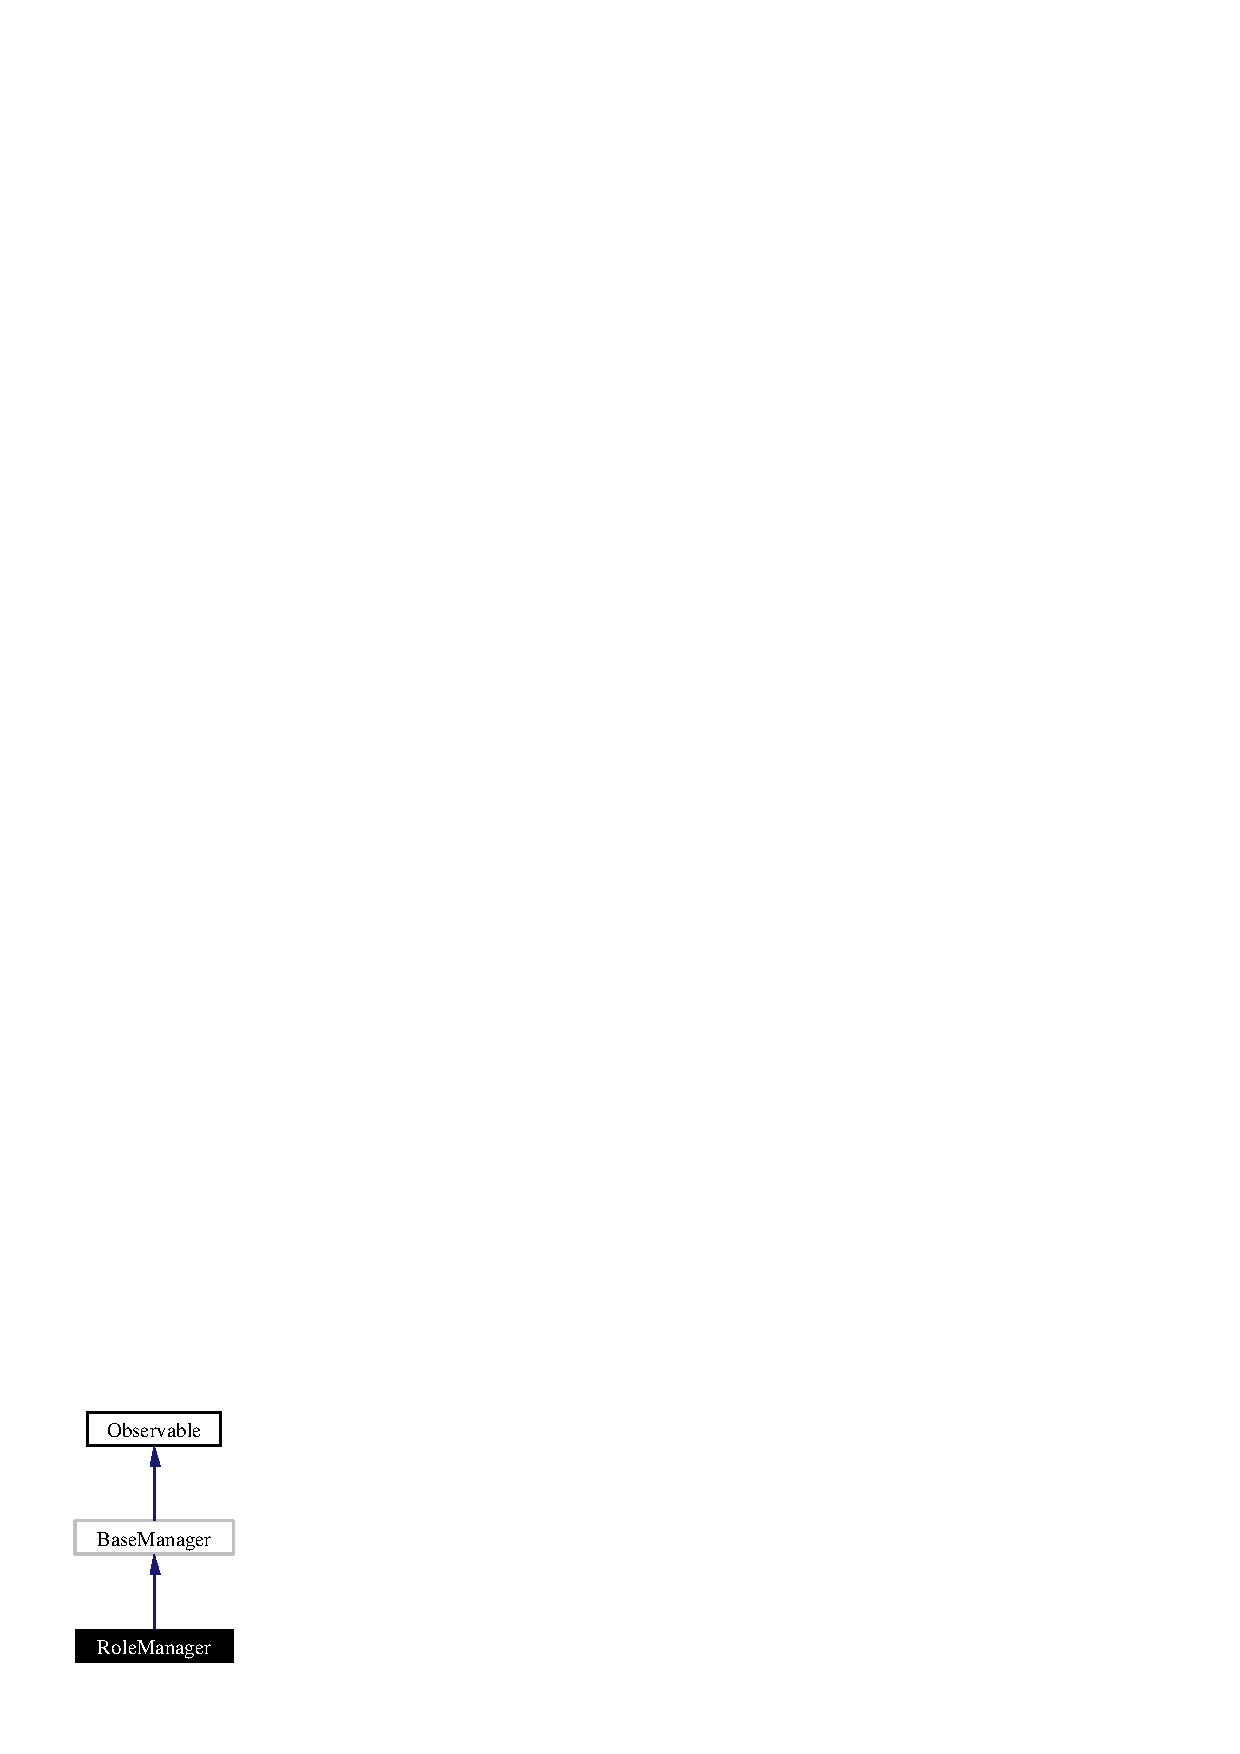
\includegraphics[width=56pt]{classRoleManager__coll__graph}
\end{center}
\end{figure}
\subsection*{Public Member Functions}
\begin{CompactItemize}
\item 
{\bf Role\-Manager} (\$db)
\item 
{\bf get\_\-role} (\$p\-Id,\$role\-Id)
\item 
{\bf map\_\-user\_\-to\_\-role} (\$p\-Id,\$user,\$role\-Id)
\item 
{\bf remove\_\-mapping} (\$user,\$role\-Id)
\item 
{\bf list\_\-mappings} (\$p\-Id,\$offset,\$max\-Records,\$sort\_\-mode,\$find)
\item 
{\bf list\_\-roles} (\$p\-Id,\$offset,\$max\-Records,\$sort\_\-mode,\$find,\$where='')
\item 
{\bf remove\_\-role} (\$p\-Id,\$role\-Id)
\item 
{\bf replace\_\-role} (\$p\-Id,\$role\-Id,\$vars)
\item 
{\bf Role\-Manager} (\$db)
\item 
{\bf get\_\-role} (\$p\-Id,\$role\-Id)
\item 
{\bf role\_\-name\_\-exists} (\$name)
\item 
{\bf map\_\-user\_\-to\_\-role} (\$p\-Id,\$user,\$role\-Id)
\item 
{\bf remove\_\-mapping} (\$user,\$role\-Id)
\item 
{\bf list\_\-mappings} (\$p\-Id,\$offset,\$max\-Records,\$sort\_\-mode,\$find)
\item 
{\bf list\_\-roles} (\$p\-Id,\$offset,\$max\-Records,\$sort\_\-mode,\$find,\$where='')
\item 
{\bf remove\_\-role} (\$p\-Id,\$role\-Id)
\item 
{\bf replace\_\-role} (\$p\-Id,\$role\-Id,\$vars)
\end{CompactItemize}


\subsection{Detailed Description}
TODO Add a method to check if a role name exists in a process (to be used to prevent duplicate names) 



Definition at line 17 of file Process\-Manager/Role\-Manager.php.

\subsection{Constructor \& Destructor Documentation}
\index{RoleManager@{Role\-Manager}!RoleManager@{RoleManager}}
\index{RoleManager@{RoleManager}!RoleManager@{Role\-Manager}}
\subsubsection{\setlength{\rightskip}{0pt plus 5cm}Role\-Manager::Role\-Manager (\$ {\em db})}\label{classRoleManager_a0}


Constructor takes a PEAR::Db object to be used to manipulate roles in the database. 

Definition at line 23 of file Process\-Manager/Role\-Manager.php.\index{RoleManager@{Role\-Manager}!RoleManager@{RoleManager}}
\index{RoleManager@{RoleManager}!RoleManager@{Role\-Manager}}
\subsubsection{\setlength{\rightskip}{0pt plus 5cm}Role\-Manager::Role\-Manager (\$ {\em db})}\label{classRoleManager_a8}


Constructor takes a PEAR::Db object to be used to manipulate roles in the database. 

Definition at line 23 of file src/Process\-Manager/Role\-Manager.php.

\subsection{Member Function Documentation}
\index{RoleManager@{Role\-Manager}!get_role@{get\_\-role}}
\index{get_role@{get\_\-role}!RoleManager@{Role\-Manager}}
\subsubsection{\setlength{\rightskip}{0pt plus 5cm}Role\-Manager::get\_\-role (\$ {\em p\-Id}, \$ {\em role\-Id})}\label{classRoleManager_a9}


Gets a role fields are returned as an asociative array 

Definition at line 34 of file src/Process\-Manager/Role\-Manager.php.\index{RoleManager@{Role\-Manager}!get_role@{get\_\-role}}
\index{get_role@{get\_\-role}!RoleManager@{Role\-Manager}}
\subsubsection{\setlength{\rightskip}{0pt plus 5cm}Role\-Manager::get\_\-role (\$ {\em p\-Id}, \$ {\em role\-Id})}\label{classRoleManager_a1}


Gets a role fields are returned as an asociative array 

Definition at line 34 of file Process\-Manager/Role\-Manager.php.\index{RoleManager@{Role\-Manager}!list_mappings@{list\_\-mappings}}
\index{list_mappings@{list\_\-mappings}!RoleManager@{Role\-Manager}}
\subsubsection{\setlength{\rightskip}{0pt plus 5cm}Role\-Manager::list\_\-mappings (\$ {\em p\-Id}, \$ {\em offset}, \$ {\em max\-Records}, \$ {\em sort\_\-mode}, \$ {\em find})}\label{classRoleManager_a13}


List mappings 

Definition at line 72 of file src/Process\-Manager/Role\-Manager.php.\index{RoleManager@{Role\-Manager}!list_mappings@{list\_\-mappings}}
\index{list_mappings@{list\_\-mappings}!RoleManager@{Role\-Manager}}
\subsubsection{\setlength{\rightskip}{0pt plus 5cm}Role\-Manager::list\_\-mappings (\$ {\em p\-Id}, \$ {\em offset}, \$ {\em max\-Records}, \$ {\em sort\_\-mode}, \$ {\em find})}\label{classRoleManager_a4}


List mappings 

Definition at line 63 of file Process\-Manager/Role\-Manager.php.\index{RoleManager@{Role\-Manager}!list_roles@{list\_\-roles}}
\index{list_roles@{list\_\-roles}!RoleManager@{Role\-Manager}}
\subsubsection{\setlength{\rightskip}{0pt plus 5cm}Role\-Manager::list\_\-roles (\$ {\em p\-Id}, \$ {\em offset}, \$ {\em max\-Records}, \$ {\em sort\_\-mode}, \$ {\em find}, \$ {\em where} = '')}\label{classRoleManager_a14}


Lists roles at a per-process level 

Definition at line 96 of file src/Process\-Manager/Role\-Manager.php.\index{RoleManager@{Role\-Manager}!list_roles@{list\_\-roles}}
\index{list_roles@{list\_\-roles}!RoleManager@{Role\-Manager}}
\subsubsection{\setlength{\rightskip}{0pt plus 5cm}Role\-Manager::list\_\-roles (\$ {\em p\-Id}, \$ {\em offset}, \$ {\em max\-Records}, \$ {\em sort\_\-mode}, \$ {\em find}, \$ {\em where} = '')}\label{classRoleManager_a5}


Lists roles at a per-process level 

Definition at line 87 of file Process\-Manager/Role\-Manager.php.\index{RoleManager@{Role\-Manager}!map_user_to_role@{map\_\-user\_\-to\_\-role}}
\index{map_user_to_role@{map\_\-user\_\-to\_\-role}!RoleManager@{Role\-Manager}}
\subsubsection{\setlength{\rightskip}{0pt plus 5cm}Role\-Manager::map\_\-user\_\-to\_\-role (\$ {\em p\-Id}, \$ {\em user}, \$ {\em role\-Id})}\label{classRoleManager_a11}


Maps a user to a role 

Definition at line 54 of file src/Process\-Manager/Role\-Manager.php.\index{RoleManager@{Role\-Manager}!map_user_to_role@{map\_\-user\_\-to\_\-role}}
\index{map_user_to_role@{map\_\-user\_\-to\_\-role}!RoleManager@{Role\-Manager}}
\subsubsection{\setlength{\rightskip}{0pt plus 5cm}Role\-Manager::map\_\-user\_\-to\_\-role (\$ {\em p\-Id}, \$ {\em user}, \$ {\em role\-Id})}\label{classRoleManager_a2}


Maps a user to a role 

Definition at line 45 of file Process\-Manager/Role\-Manager.php.\index{RoleManager@{Role\-Manager}!remove_mapping@{remove\_\-mapping}}
\index{remove_mapping@{remove\_\-mapping}!RoleManager@{Role\-Manager}}
\subsubsection{\setlength{\rightskip}{0pt plus 5cm}Role\-Manager::remove\_\-mapping (\$ {\em user}, \$ {\em role\-Id})}\label{classRoleManager_a12}


Removes a mapping 

Definition at line 63 of file src/Process\-Manager/Role\-Manager.php.\index{RoleManager@{Role\-Manager}!remove_mapping@{remove\_\-mapping}}
\index{remove_mapping@{remove\_\-mapping}!RoleManager@{Role\-Manager}}
\subsubsection{\setlength{\rightskip}{0pt plus 5cm}Role\-Manager::remove\_\-mapping (\$ {\em user}, \$ {\em role\-Id})}\label{classRoleManager_a3}


Removes a mapping 

Definition at line 54 of file Process\-Manager/Role\-Manager.php.\index{RoleManager@{Role\-Manager}!remove_role@{remove\_\-role}}
\index{remove_role@{remove\_\-role}!RoleManager@{Role\-Manager}}
\subsubsection{\setlength{\rightskip}{0pt plus 5cm}Role\-Manager::remove\_\-role (\$ {\em p\-Id}, \$ {\em role\-Id})}\label{classRoleManager_a15}


Removes a role. 

Definition at line 126 of file src/Process\-Manager/Role\-Manager.php.\index{RoleManager@{Role\-Manager}!remove_role@{remove\_\-role}}
\index{remove_role@{remove\_\-role}!RoleManager@{Role\-Manager}}
\subsubsection{\setlength{\rightskip}{0pt plus 5cm}Role\-Manager::remove\_\-role (\$ {\em p\-Id}, \$ {\em role\-Id})}\label{classRoleManager_a6}


Removes a role. 

Definition at line 117 of file Process\-Manager/Role\-Manager.php.\index{RoleManager@{Role\-Manager}!replace_role@{replace\_\-role}}
\index{replace_role@{replace\_\-role}!RoleManager@{Role\-Manager}}
\subsubsection{\setlength{\rightskip}{0pt plus 5cm}Role\-Manager::replace\_\-role (\$ {\em p\-Id}, \$ {\em role\-Id}, \$ {\em vars})}\label{classRoleManager_a16}


Updates or inserts a new role in the database, \$vars is an asociative array containing the fields to update or to insert as needed. \$p\-Id is the process\-Id \$role\-Id is the role\-Id 

Definition at line 142 of file src/Process\-Manager/Role\-Manager.php.\index{RoleManager@{Role\-Manager}!replace_role@{replace\_\-role}}
\index{replace_role@{replace\_\-role}!RoleManager@{Role\-Manager}}
\subsubsection{\setlength{\rightskip}{0pt plus 5cm}Role\-Manager::replace\_\-role (\$ {\em p\-Id}, \$ {\em role\-Id}, \$ {\em vars})}\label{classRoleManager_a7}


Updates or inserts a new role in the database, \$vars is an asociative array containing the fields to update or to insert as needed. \$p\-Id is the process\-Id \$role\-Id is the role\-Id 

Definition at line 133 of file Process\-Manager/Role\-Manager.php.\index{RoleManager@{Role\-Manager}!role_name_exists@{role\_\-name\_\-exists}}
\index{role_name_exists@{role\_\-name\_\-exists}!RoleManager@{Role\-Manager}}
\subsubsection{\setlength{\rightskip}{0pt plus 5cm}Role\-Manager::role\_\-name\_\-exists (\$ {\em name})}\label{classRoleManager_a10}


Indicates if a role exists 

Definition at line 45 of file src/Process\-Manager/Role\-Manager.php.

The documentation for this class was generated from the following files:\begin{CompactItemize}
\item 
Process\-Manager/Role\-Manager.php\item 
src/Process\-Manager/Role\-Manager.php\end{CompactItemize}
